\documentclass[12pt, letterpaper, twoside]{article}
\usepackage[utf8]{inputenc}
\usepackage[a4paper]{geometry}
\usepackage{array}
\usepackage{booktabs} % For prettier tables
\usepackage{multirow}
\usepackage{multicol}
\usepackage{ragged2e}
\usepackage{xcolor}
\usepackage{gensymb}
\usepackage{fullpage}
\usepackage{hyperref}
\usepackage{amsmath}
\usepackage{scrextend}
\usepackage{graphicx}

\graphicspath{ {./bilder/} }
\newcommand{\cfootnote}[1]{\footnote{\centering #1}}
\title{Bac 2014 Uppgift A1}
\author{Simon Freiermuth \\ \href{mailto:simon@freiermuth.org}{simon@freiermuth.org}}
\date{16 April, 2020}

\begin{document}

%\begin{titlepage}
\maketitle
%\end{titlepage}

\begin{flushleft}

%%%%%%%%%%%%%%%%%%%%%%%%%%%%%%%%%%%%%%%%%%%%%%%%%%%%%%%%%%%%%%%%%%%%%%%%%
%%%%%%%%%%%%%%%%%%%%%%%%%%%%%%%%%%%%%%%%%%%%%%%%%%%%%%%%%%%%%%%%%%%%%%%%%%
%                   Begin
%%%%%%%%%%%%%%%%%%%%%%%%%%%%%%%%%%%%%%%%%%%%%%%%%%%%%%%%%%%%%%%%%%%%%%%%%
%%%%%%%%%%%%%%%%%%%%%%%%%%%%%%%%%%%%%%%%%%%%%%%%%%%%%%%%%%%%%%%%%%%%%%%%%%
%%%%%%%%%%%%%%%%%%%%%%%%%%%%%%%%%%%%%%%%%%%%%%%%%%%%%%%%%%%%%%%%%%%%%%%%%%
%                   Deluppgift b)
%%%%%%%%%%%%%%%%%%%%%%%%%%%%%%%%%%%%%%%%%%%%%%%%%%%%%%%%%%%%%%%%%%%%%%%%%
\begin{itemize}
%
\item[\textbf{a)}]En \textbf{stark} enprotonig syra $ HX $, är i fast form vid $ 25\ \degree C $.
Syran är den enda sura beståndsdelen i ett avkalkningsmedel för kaffemaskiner.
Antag att kalkavlagringarna i kaffemaskinen består av $ CaCO_3(s) $,
och ange ekvationen för reaktionen som kan observeras när avkalkaren gör sitt jobb.
\newline
\newline
$ CaCO_3(s)\ \overset{H_2O}{\rightarrow}\ Ca^{2+}(aq)\ +\ CO_3^{2-}(aq) $

$ 2HX(aq)\ +\ CaCO_3(s)\ \rightarrow\ H_2CO_3\ +\ Ca^{2+} + 2X^- $
\newline
%%%%%%%%%%%%%%%%%%%%%%%%%%%%%%%%%%%%%%%%%%%%%%%%%%%%%%%%%%%%%%%%%%%%%%%%%%
%                   Deluppgift b)
%%%%%%%%%%%%%%%%%%%%%%%%%%%%%%%%%%%%%%%%%%%%%%%%%%%%%%%%%%%%%%%%%%%%%%%%%%
\item[\textbf{b)}]En kommersiell avkalkningsprodukt innehåller 91.0\%\ $ HX $ (massprocent).

För att kunna bestämma molmassan löser man upp $ 3.00\ g $ av avkalkaren i $ 5.00*10^{-1}\ dm^3 $ destillerat vatten.
Ett prov på $ 20.0\ cm^3 $ titreras med en natriumhydroxid-lösning,
$ NaOH(aq) $. Lösningens pH antecknas samtidigt som den tillsatta basens volym, $ V_b $, stiger progressivt.
\newline
\newline
Den resulterande graphen, $ pH=f(V_b) $ gav följande information:\\
\begin{addmargin}[1em]{2em}% 1em left, 2em right
    $ pH = 1.25\ n\ddot{a}r\ V_b = 0.00\ cm^3 $

    $ pH = 7.00\ n\ddot{a}r\ V_b = 11.2\ cm^3 $

\end{addmargin}
\hfill
%%%%%%%%%%%%%%%%%%%%%%%%%%%%%%%%%%%%%%%%%%%%%%%%%%%%%%%%%%%%%%%%%%%%%%%%%%
%                   Deluppgift i.
%%%%%%%%%%%%%%%%%%%%%%%%%%%%%%%%%%%%%%%%%%%%%%%%%%%%%%%%%%%%%%%%%%%%%%%%%%
\begin{itemize}
\item[\textbf{i.}] Skissa den resulterande titreringsgrafen.
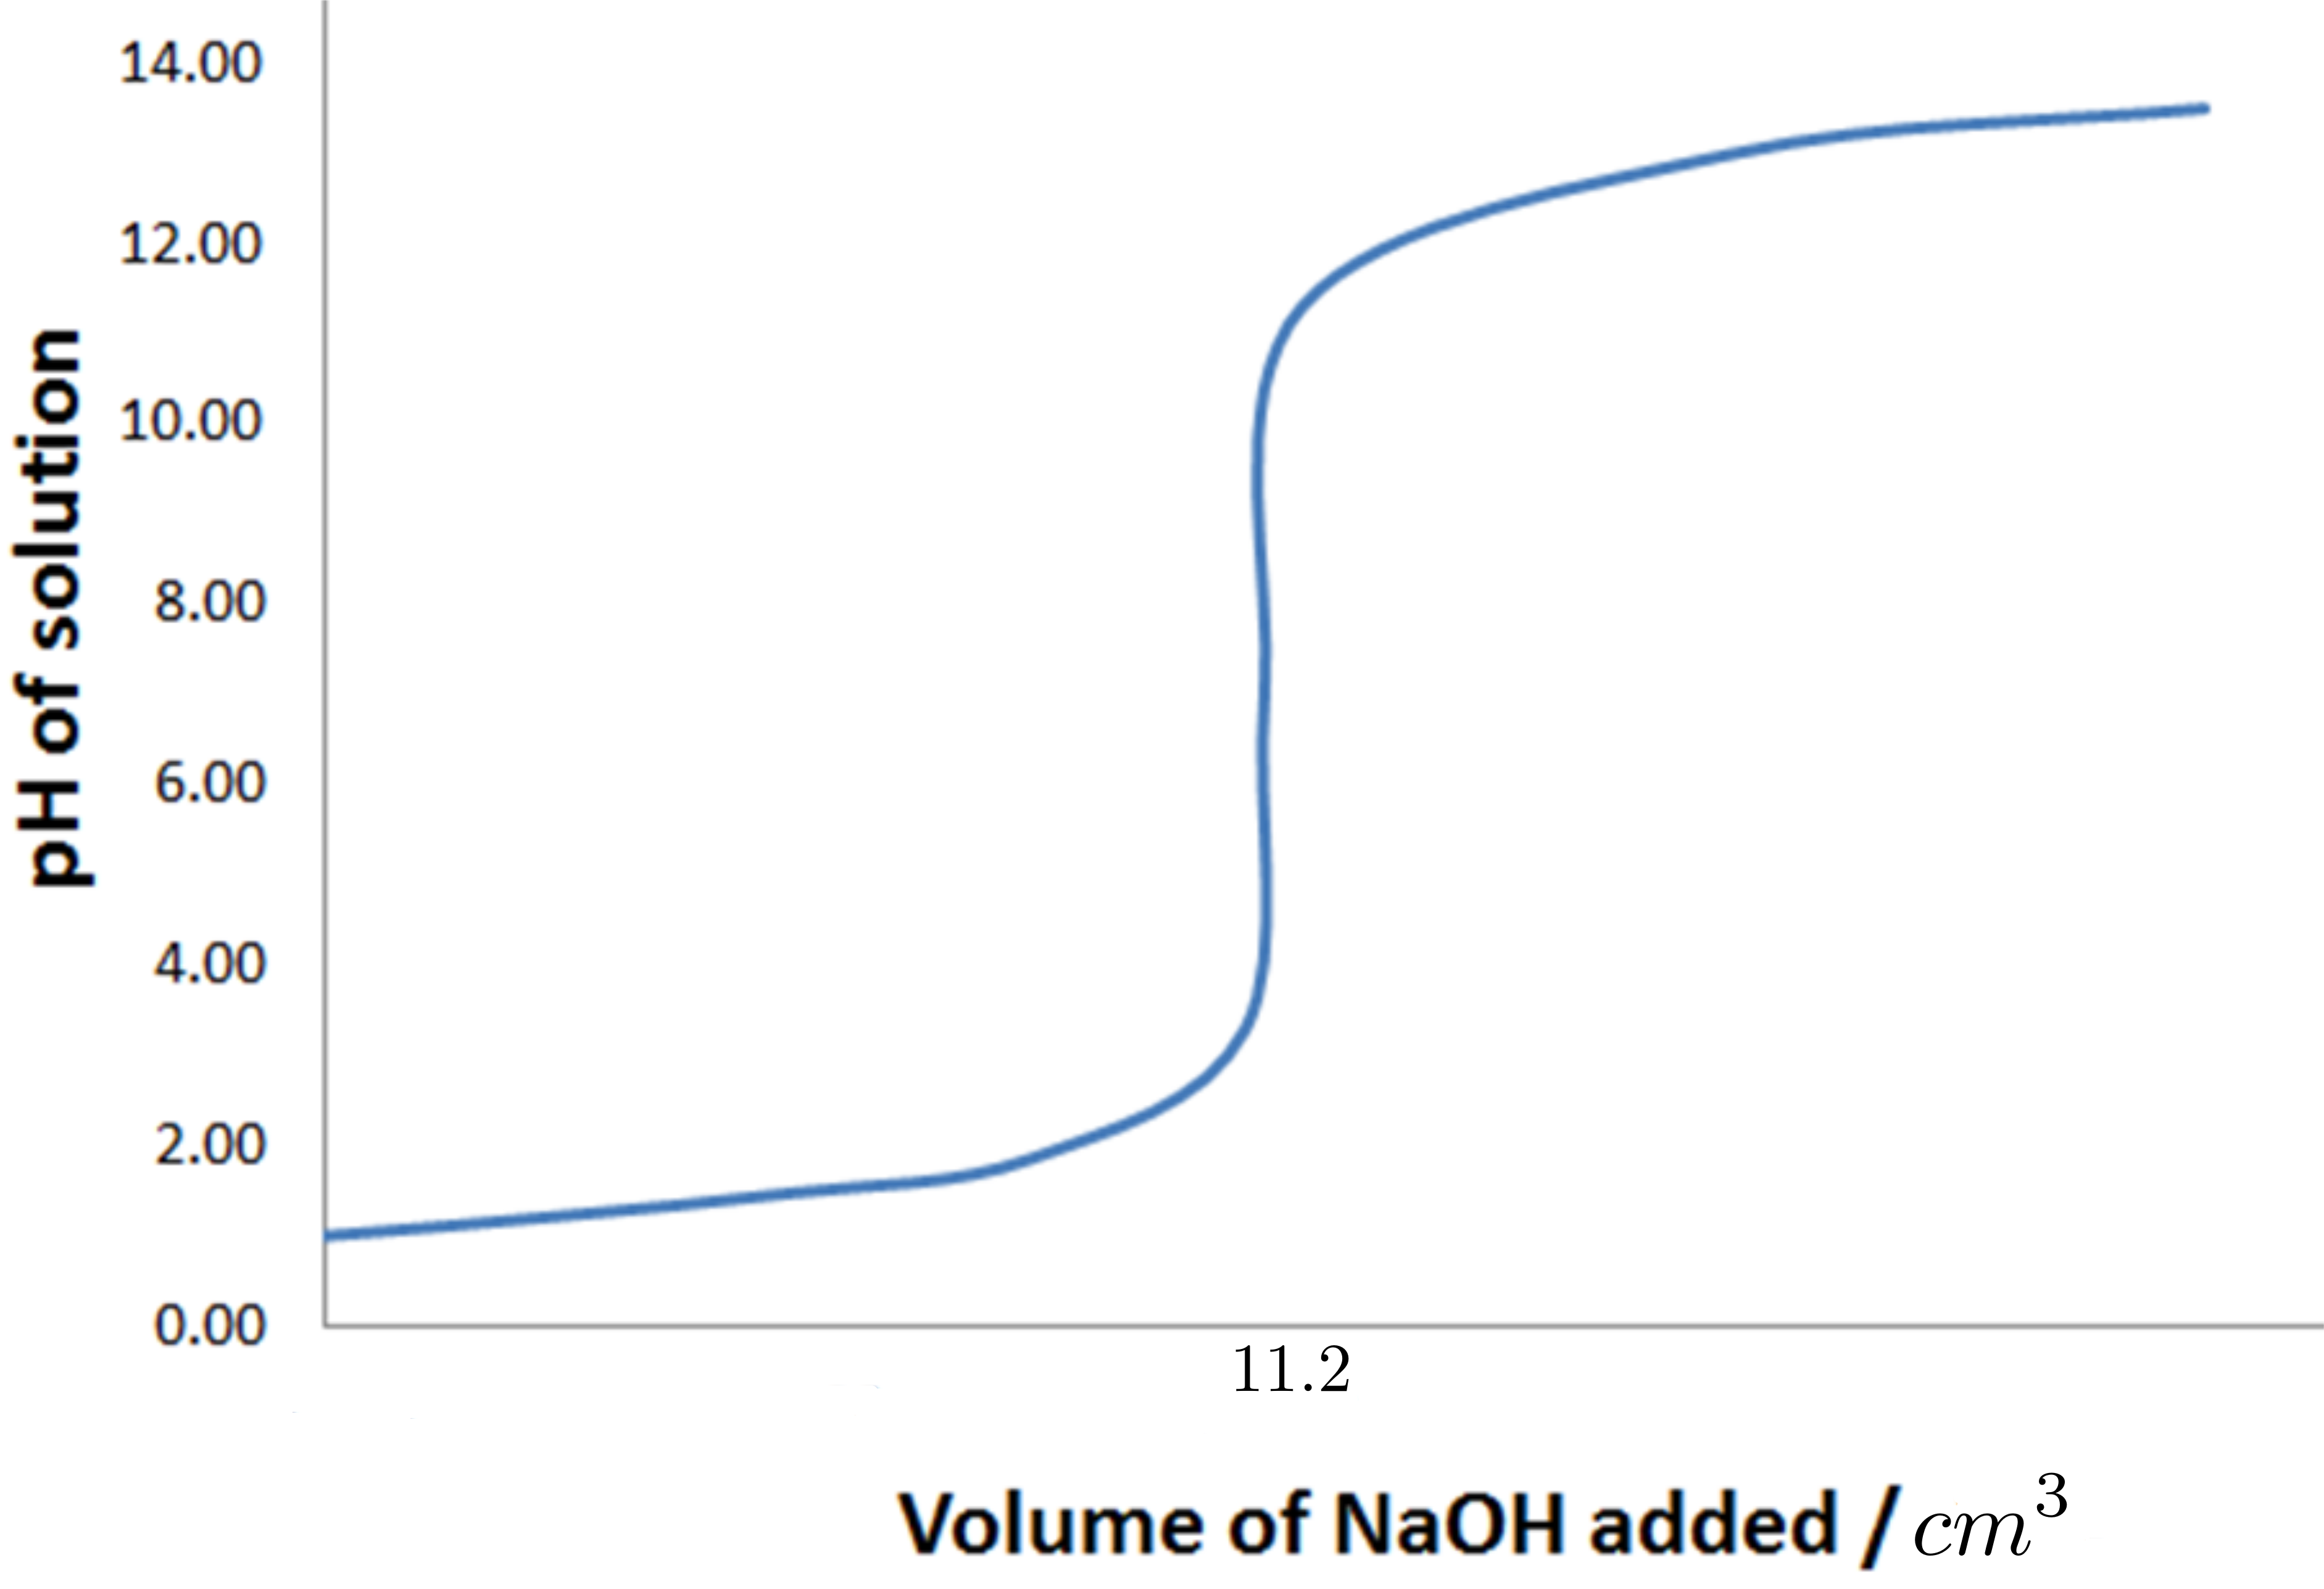
\includegraphics[scale=0.07]{ph_curve}
\hfill
%%%%%%%%%%%%%%%%%%%%%%%%%%%%%%%%%%%%%%%%%%%%%%%%%%%%%%%%%%%%%%%%%%%%%%%%%%
%                   Deluppgift ii.
%%%%%%%%%%%%%%%%%%%%%%%%%%%%%%%%%%%%%%%%%%%%%%%%%%%%%%%%%%%%%%%%%%%%%%%%%%
\item[\textbf{ii.}] Visa med hjälp av en uträkning att den initiala koncentrationen av syran är $ 5.62*10^{-2}\ mol/dm^3 $

$ pH=-log([H^+]) $

$ C_{init}(HX)=10^{-1.25}\ =\ 5.62*10^{-2}\ mol/dm^{-3} $

Eftersom syran är stark dissocieras den fullständigt: $ [H^+] = C_{init}(HX) $

%\pagebreak

%%%%%%%%%%%%%%%%%%%%%%%%%%%%%%%%%%%%%%%%%%%%%%%%%%%%%%%%%%%%%%%%%%%%%%%%%%
%                   Deluppgift iii.
%%%%%%%%%%%%%%%%%%%%%%%%%%%%%%%%%%%%%%%%%%%%%%%%%%%%%%%%%%%%%%%%%%%%%%%%%%
\item[\textbf{iii.}] Beräkna molmassan av syran $ HX $.

$ n=C*V $

$ n(HX)=10^{-1.25}*0.5 = 0.028117\ mol $
\newline
\newline
$ n=\frac{m}{M}\ \rightarrow\ M=\frac{m}{n} $

$ m(HX)=m(Avkalkare)*0.91 $

$ m(HX)=3.00*0.91=2.73\ g $

$ M(HX)=\frac{2.73}{0.028117}=97.0942845965\ g/mol $

\hfill
%%%%%%%%%%%%%%%%%%%%%%%%%%%%%%%%%%%%%%%%%%%%%%%%%%%%%%%%%%%%%%%%%%%%%%%%%%
%                  Deluppgift iv.
%%%%%%%%%%%%%%%%%%%%%%%%%%%%%%%%%%%%%%%%%%%%%%%%%%%%%%%%%%%%%%%%%%%%%%%%%%
\item[\textbf{iv.}] Beräkna koncentrationen av $ NaOH(aq) $

$ HX\ +\ NaOH\ \rightarrow\ Na^+\ +\ X^-\ +\ H_2O $

$ V_{eq}(NaOH(aq))\ =\ 11.2\ cm^3 $

$ n_{init}(HX)=n_{eq}(OH^-) $

$ n_{init}(HX)= 10^{-1.25}*0.02=0.0011247\ mol $

$ n_{eq}(OH^-)\ =\ 1.13*10^{-3}\ mol $

$ C=\frac{n}{V} $

$ C(OH^-)\ =\ \frac{1.13*10^{-3}}{0.0112}\ =\ 0.01\ mol/dm^3 $

\hfill
%%%%%%%%%%%%%%%%%%%%%%%%%%%%%%%%%%%%%%%%%%%%%%%%%%%%%%%%%%%%%%%%%%%%%%%%%%
%                   Deluppgift v.
%%%%%%%%%%%%%%%%%%%%%%%%%%%%%%%%%%%%%%%%%%%%%%%%%%%%%%%%%%%%%%%%%%%%%%%%%%
\item[\textbf{v.}] Hitta molekylformeln för syran $ HX $.

\hfill

Fler experiment har igenomförts för att bestämma den procentuella sammansättningen
av massan av varje element i syran $ HX $. Följande resultat har noterats:\\

\hfill

$ H:\ 3.10\%,\ N:\ 14.4\%,\ S:\ 33.3\%,\ O:\ 49.5\% $



Vi utgår ifrån $ 100 g $

\renewcommand{\arraystretch}{1.5}
\begin{tabular}{ |c|c|c|c|c| }
 \hline
  & $ H $ & $ N $ & $ S $ & $ O $ \\
 \hline
 Massprocent & $ 3.10\% $ & $ 14.4\% $ & $ 33.3\% $ & $ 49.5\% $ \\
 \hline
 Antal $ g $ & $ 3.10\ g $ & $ 14.4\ g $ & $ 33.3\ g $ & $ 49.5\ g $ \\
 \hline
 Antal $ mol $ & $ \frac{3.10}{1.01}=3.07\ $ & $ \frac{14.4}{14.0}=1.03 $ & $ \frac{33.3}{32.1}=1.04 $ & $ \frac{49.5}{16.0}=3.09 $ \\
 \hline
\end{tabular}


\footnote{
\textbf{Givet:} $ K_w=1.00*10^{-14} $\\
Molmassa (i $ g*mol^{-1} $):\\
$ H:\ 1.01;\ O:\ 16.0;\ N:\ 14.0;\ S:\ 32.1 $
}

\pagebreak
\hfill

$ H_{3.07}N_{1.03}S_{1.04}O_{3.09}\ \rightarrow\ NH_3SO_3 $

$ M_{empirisk}(NH_3SO_3)\ =\ 14+3*1+32+3*16 = 97\ g/mol $

$ M(HX)\ =\ 97\ g/mol:\ \rightarrow\ NH_3SO_3 $ är den riktiga molekylformeln.



%$ n=\frac{m}{M} $

%NU HAR VI MER TID TILL ATT RITA KEMISKA FIGURER OCH SÅNT
%\hfill

%asSÅ dÅ fÅR VI MER TID ÖVER SLIPPER SOCKER MOLEKYLERNA... FÖR DET HADE VI KVAR. o

\end{itemize}


%%%%%%%%%%%%%%%%%%%%%%%%%%%%%%%%%%%%%%%%%%%%%%%%%%%%%%%%%%%%%%%%%%%%%%%%%%
%                   Deluppgift c)
%%%%%%%%%%%%%%%%%%%%%%%%%%%%%%%%%%%%%%%%%%%%%%%%%%%%%%%%%%%%%%%%%%%%%%%%%%
\item[\textbf{c)}] Ett annat avkalkningsmedel är en enprotonig syra, $ HY $.
Den har studerats med en liknande metod.

Man löser $ 3.00\ g $ rent $ HY $ i $ 5.00*10^{-1}\ dm^3 $ destillerat vatten. $ 20.0\ cm^3 $ av den här
lösningen titrerades med en lösning av natriumhydroxid, $ NaOH(aq) $. pH mättes i jämna intervall samtidigt
som basen tillsattes. En graph plottades: $ f(V_b)\ =\ pH $.

Den resulterande grafen visar att $ HY $ är en svag syra och gav följande information:

$ pH\ =\ 2.90\ n\ddot{a}r\ V_b\ =\ 0.00\ cm^3 $

$ pH\ vid\ halvekvivalenspunkten:\ 4.80 $


\begin{itemize}
%%%%%%%%%%%%%%%%%%%%%%%%%%%%%%%%%%%%%%%%%%%%%%%%%%%%%%%%%%%%%%%%%%%%%%%%%%
%                   Deluppgift i.
%%%%%%%%%%%%%%%%%%%%%%%%%%%%%%%%%%%%%%%%%%%%%%%%%%%%%%%%%%%%%%%%%%%%%%%%%%
\item[\textbf{i.}] Beräkna den \textbf{initiala} koncentrationen av syran $ HY $.

$ pH\ =\ pK_a\ +\ log(\frac{[A^-]}{[HA]}) $

$ pH_{\frac{1}{2}eq}\ =\ pK_a $

$ pK_a\ =\ 4.80 $

$ pH\ =\ -log([H^+]) $

$ [H^+]\ =\ 10^{-2.90}\ mol/dm^3 $

\hfill
\hfill

\renewcommand{\arraystretch}{1.5}
\begin{tabular}{ |c|c|c|c| }
 \hline
   & \multicolumn{3}{c|}{ $ HY\ +\ H_2O\ \rightleftharpoons\ H_3O^+(aq)\ +\ Y^-(aq) $} \\
 \hline
 I & \hspace{1.25cm} $ x $ \hspace{1.2cm} & $ - $ & $ - $ \\
 \hline
 C & $ -10^{-2.90} $ & $ +10^{-2.90} $ & $ +10^{-2.90} $ \\
 \hline
 E & $ x-10^{-2.90} $ & \hspace{0.4cm} $ 10^{-2.90} $ \hspace{0.4cm} & $ 10^{-2.90} $ \\
 \hline
\end{tabular}

\hfill

$ K_a\ =\ \frac{[H_3O^+(aq)]*[Y^-(aq)]}{[HY]} $

$ 10^{-4.80} = \frac{(10^{-2.90})^2}{x-10^{-2.90}} $

$ 10^{-4.80} = \frac{10^{-2.90+(-2.90)}}{x-10^{-2.90}} $

$ x-10^{-2.90} = \frac{10^{-5.80}}{10^{-4.80}} $

$ x = 10^{-5.80-(-4.80)}+10^{-2.90} $

$ x = 0.1013\ mol/dm^3 $

\pagebreak

\item[\textbf{ii.}] Visa med beräkning att pH vid ekvivalenspunkten är 8.75,
efter att man har lagt till $ 20.0\ cm^3\ NaOH(aq) $.

\hfill
\hfill

$ n_{init}(HY)\ =\ C_{init}(HY)\ *\ V_{init} $

$ n_{init}(HY)\ =\ 0.1013*0.02=0.002025\ mol $

$ n_{init}(HY)\ =\ n_{eq}(Y^-) $

$ C_{eq}(Y^-)\ =\ \frac{n_{eq}(Y^-)}{V_{eq}} $

$ C_{eq}(Y^-)\ =\ \frac{0.002025}{0.04}\ =\ 0.050625\ mol/dm^3 $

\hfill

ICE tabell i $ mol/dm^3 $

\renewcommand{\arraystretch}{1.5}
\begin{tabular}{ |c|c|c|c| }
 \hline
 Volym: $ 0.04\ dm^3 $  & \multicolumn{3}{c|}{ $Y^-\ +\ H_2O\ \rightleftharpoons\ OH^-\ \ \ \ +\ \ HY $  } \\
 \hline
 I & \hspace{0.5cm} $ 0.050625 $ \hspace{0.5cm} & \hspace{0.3cm} $ - $ \hspace{0.3cm} & $ - $ \\
 \hline
 C & $ -x $ & $ +x $ & $ +x $ \\
 \hline
 E & $ 0.050625-x $ & $ x $ & $ x $ \\
 \hline
\end{tabular}

$ K_a\ =\ 10^{-4.80} $

$ K_b\ =\ 10^{-14}\ =\ 10^{-4.80} $

$ K_b\ =\ \frac{[HY]*[OH^-]}{[Y^-]} $

$ 10^{-(14-4.80)} \ =\ \frac{x^2}{0.050625-x} $

$ x=5.6514*10^{-6}\ =\ [OH^-] $

$ pOH\ =\ -log([OH^-]) $

$ pH\ =\ 14-pOH $

$ pH\ =\ 14-(-log(5.6514*10^{-6})j\ =\ 8.75216 $

\hfill


\item[\textbf{iii.}] Beskriv hur titrergraphen med en stark syra och en stark bas skiljer
sig ifrån en graf med en svag syra och en stark bas.

\hfill

I en titrering med en stark syra och en stark bas finns ingen buffertzon. (se graf i uppgift A1, b), i. )

En titrering med en svag syra och en stark bas har en buffertzon, dvs man måste hälla på ett tag innan man
plötsligt når jämnvikten.

Ekvivalenspunkten nås vid olika pH eftersom den svaga syrans konjugerande bas är en stark bas.


\end{itemize}
\pagebreak
\item[\textbf{d)}] Båda syrorna $ HX $, och $ HY $ kan användas i en buffertlösning när man blandar dem med
en annan substans in vatten.

\begin{itemize}

\item[\textbf{i.}] Visa hur det här kan uppnås med var och en av syrorna.

\hfill

Har man $ HX $, en stark syra, kan man lägga till den i en svag bas, då kommer allt $ HX $
reagera och den svaga basen bilda en svag konjugerande syra.

\hfill

Har man $ HY $, en svag syra, kan man lägga till en stark bas, då kommer en del av $ HY $
reagera och bilda den konjugerande basen $ Y^- $.

\hfill

\item[\textbf{ii.}]
Visa med hjälp av två relevanta ekvationer hur en bufferlösning med $ HY $ kan buffra.

\hfill

Våran bufferlösning: \\
$ HY\ +\ H_2O\ \rightleftharpoons\ Y^-\ +\ H_3O^+ $

\hfill

Har man alltså 1 mol HY lägger man till 0.5 mol stark bas, och delar därmed upp antal mol $ HY $
i två delar, $ HY $ och $ Y^- $.

Vi får då en jämnvikt mellan $ HY $ och $ Y^- $: \\
$ \frac{[Y^-]}{[HY]}\ \approx\ 1 $

\hfill

Bufferverkan vid tillsats av bas: \\
$ HY\ +\ NaOH\ \rightarrow\ Na^+\ +\ Y^-\ +\ H_2O $

$ Y^- $ är en svag bas. Lösningen kommer att bli lite mer basisk, men det kommer inte bli
några dramatiska ändringar tills $ HY $ tar slut.

\hfill

Bufferverkan vid tillsats av syra: \\
$ Y^-\ +\ HCl\ \rightarrow\ HY\ +\ Cl^- $

$ HY $ är en svag syra. Lösningen kommer att bli lite mer sur, men det kommer inte bli
några dramatiska ändringar tills $ Y^- $ tar slut.

\end{itemize}
\end{itemize}
\end{flushleft}

%\centering\footnote{
%\textbf{Givet:} $ K_w=1.00*10^{-14} $\\
%Molmassa (i $ g*mol^{-1} $):\\
%$ H:\ 1.01;\ O:\ 16.0;\ N:\ 14.0;\ S:\ 32.1 $
%}


%%%%%%%%%%%%%%%%%%%%%%%%%%%%%%%%%%%%%%%%%%%%%%%%%%%%%%%%%%%%%%%%%%%%%%%%%%
%%%%%%%%%%%%%%%%%%%%%%%%%%%%%%%%%%%%%%%%%%%%%%%%%%%%%%%%%%%%%%%%%%%%%%%%%%
% End
%%%%%%%%%%%%%%%%%%%%%%%%%%%%%%%%%%%%%%%%%%%%%%%%%%%%%%%%%%%%%%%%%%%%%%%%%%
%%%%%%%%%%%%%%%%%%%%%%%%%%%%%%%%%%%%%%%%%%%%%%%%%%%%%%%%%%%%%%%%%%%%%%%%%%

\end{document}
